% id: 0127
% book: RPM 중3-2 수학 · 01 삼각비
% section: 중단원 마무리하기
% figure: crop:fig-0127.png
% answer: ③
% answer_source: 답지
% variant_level: 0 (원본 전사)
% 이 파일은 build.mjs 가 items.json 에서 만든다. 고칠 때는 items.json 을 고친다.
\dmkichul{RPM 중3-2 수학 0127번 · 22쪽}
\noindent\begin{minipage}[t]{0.58\linewidth}\vspace{0pt}\raggedright 오른쪽 그림과 같은 직각삼각형~$\pt{ABC}$에서 $\seg{BC}=4$이고 $\sin\pt{A}=\dfrac{\sqrt{3}}{3}$일 때, 다음 중 옳지 \underline{않은} 것은?\end{minipage}\hfill\begin{minipage}[t]{0.4\linewidth}\vspace{0pt}\centering 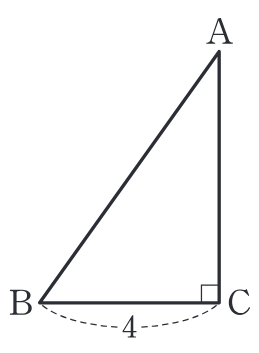
\includegraphics[width=62.1pt]{figures/fig-0127.png}\end{minipage}\par
\begin{choicesii}{\rule[-3ex]{0pt}{8ex}$\cos\pt{A}=\dfrac{\sqrt{6}}{3}$}{\rule[-3ex]{0pt}{8ex}$\tan\pt{A}=\dfrac{\sqrt{2}}{2}$}{\rule[-3ex]{0pt}{8ex}$\sin\pt{B}=\dfrac{\sqrt{3}}{2}$}{\rule[-3ex]{0pt}{8ex}$\cos\pt{B}=\dfrac{\sqrt{3}}{3}$}{\rule[-3ex]{0pt}{8ex}$\tan\pt{B}=\sqrt{2}$}\end{choicesii}
